\documentclass[10pt,aspectratio=169]{beamer}
\usepackage[utf8]{inputenc}
\usepackage[T5]{fontenc}
\usepackage{lmodern}
\usepackage[vietnamese]{babel}
\usepackage{graphicx}
\usepackage{tikz}

\usetheme{Madrid}
\usecolortheme{default}

% Customize the frametitle to include the TDTU logo at top left
\addtobeamertemplate{frametitle}{}{%
\begin{tikzpicture}[remember picture,overlay]
\node[anchor=north west, xshift=2mm, yshift=-2mm] at (current page.north west) {
\includegraphics[height=1.2cm]{image/logo-tdtu.jpg}};
\end{tikzpicture}
}

\title[Metro Ethernet MPLS]{Thiết kế và triển khai mạng Metro Ethernet sử dụng MPLS cho kết nối đa chi nhánh doanh nghiệp}
\author[N.V.T.Bảo]{Nguyễn Văn Thiên Bảo - 52300179}
\institute[TDTU]{Đại học Tôn Đức Thắng\\Khoa Công nghệ thông tin}
\date{\today}

\begin{document}

{
\setbeamertemplate{headline}{} % Hide header on title page to put logo explicitly if needed, but it's easier to just put it:
\begin{frame}
\begin{tikzpicture}[remember picture,overlay]
\node[anchor=north west, xshift=2mm, yshift=-2mm] at (current page.north west) {
\includegraphics[height=1.5cm]{image/logo-tdtu.jpg}};
\end{tikzpicture}
\titlepage
\end{frame}
}

\begin{frame}{Nội dung trình bày}
    \tableofcontents
\end{frame}

\section{Mở đầu \& Giới thiệu}
\begin{frame}{Mở đầu \& Giới thiệu}
    \begin{itemize}
        \item \textbf{Mục tiêu:} Xây dựng mô hình kết nối 3 chi nhánh doanh nghiệp qua hạ tầng mạng nhà cung cấp (Metro Ethernet).
        \item \textbf{Kiến trúc LAN đa dạng:}
        \begin{itemize}
            \item Branch 1: Flat Network (Mạng phẳng).
            \item Branch 2: Three-tier Network (Mạng 3 lớp: Access - Distribution - Core).
            \item Branch 3: Leaf-Spine Network (Mạng trung tâm dữ liệu).
        \end{itemize}
        \item \textbf{Công nghệ lõi:} Sử dụng mạng chuyển mạch nhãn đa giao thức (MPLS).
        \item \textbf{Môi trường mô phỏng:} Mininet, Open vSwitch, và Linux network namespaces.
    \end{itemize}
\end{frame}

\section{Mô hình tổng thể (Topology)}
\begin{frame}{Mô hình tổng thể (Topology)}
    \begin{columns}
        \column{0.5\textwidth}
        \begin{itemize}
            \item \textbf{Backbone Provider:} Gồm các bộ định tuyến CE (Customer Edge), PE (Provider Edge), và P (Provider).
            \item \textbf{Đường đi dữ liệu:} Lưu lượng liên chi nhánh bắt buộc phải đi qua lộ trình: CE $\rightarrow$ PE $\rightarrow$ P $\rightarrow$ PE $\rightarrow$ CE.
            \item Đảm bảo đúng chuẩn thiết kế kiến trúc mạng diện rộng (WAN/MAN).
        \end{itemize}
        \column{0.5\textwidth}
        \centering
        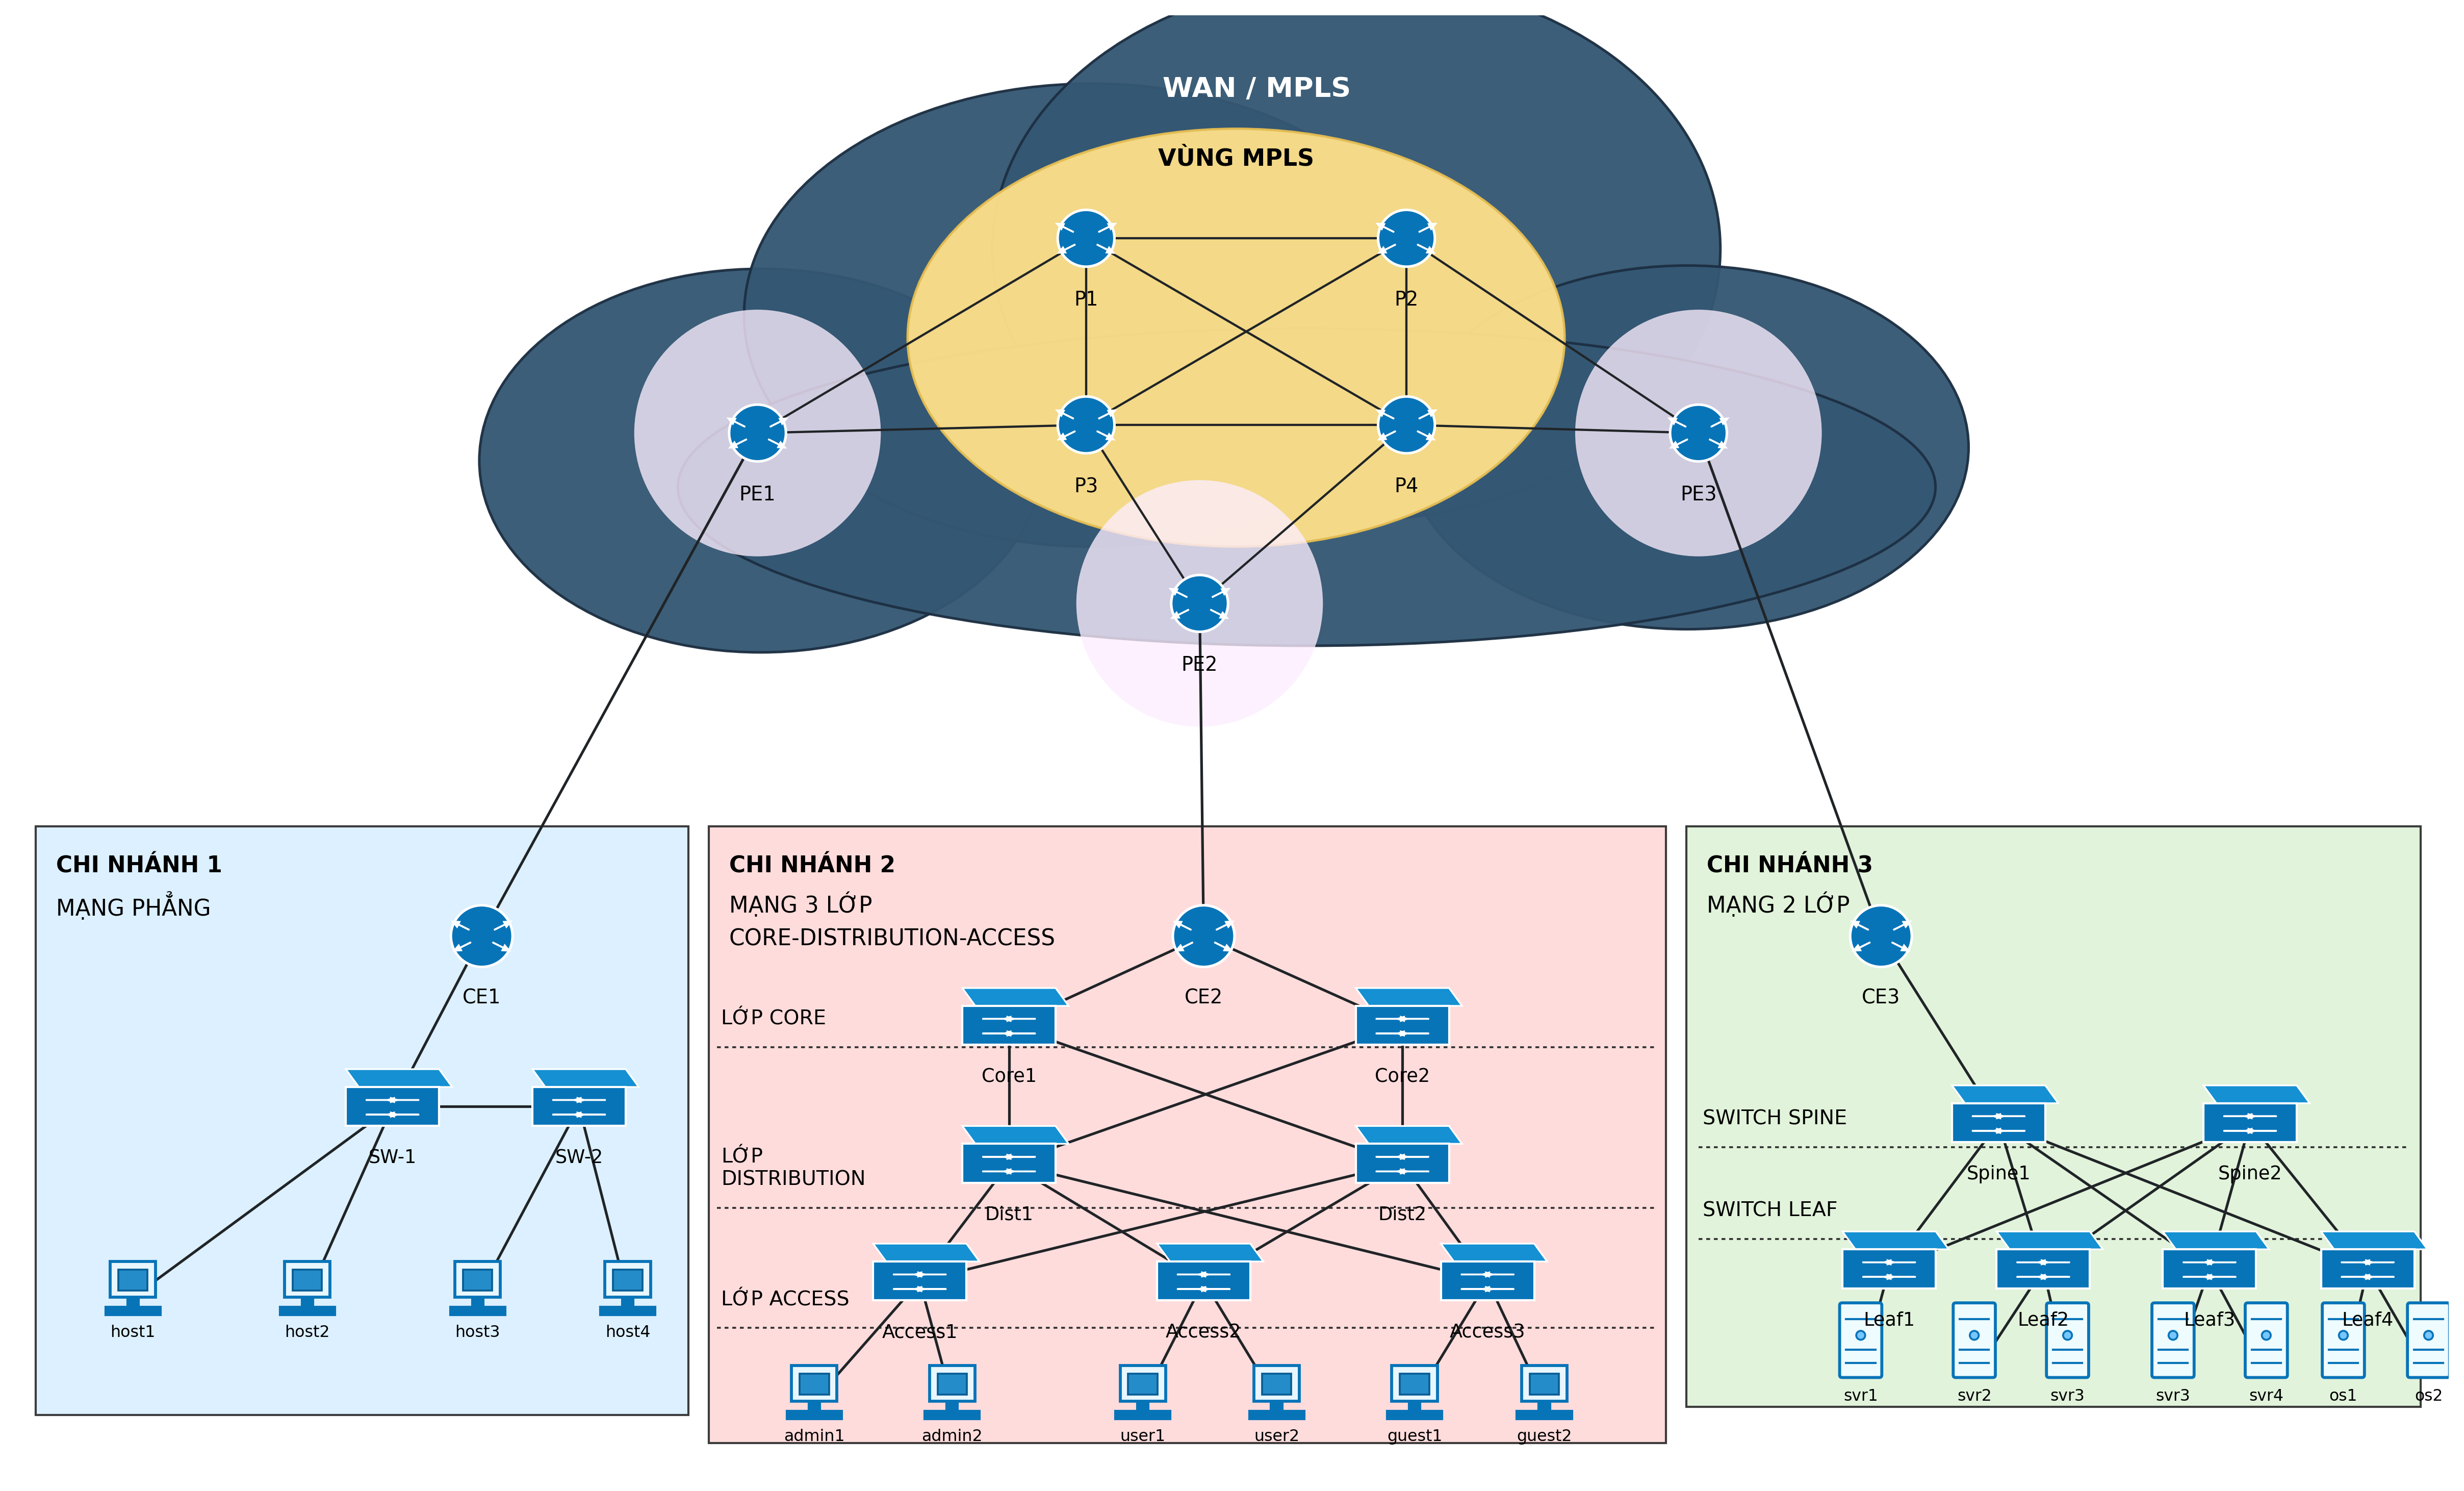
\includegraphics[width=\textwidth]{image/topology_overview.png}
    \end{columns}
\end{frame}

\section{Hoạt động của MPLS \& OSPF/LDP}
\begin{frame}{Cơ chế hoạt động của MPLS \& Control-Plane}
    \begin{block}{Quá trình chuyển tiếp bằng nhãn (MPLS Forwarding)}
        \begin{itemize}
            \item \textbf{Ingress PE:} Gán nhãn (Push label) vào gói tin.
            \item \textbf{P Router:} Hoán đổi nhãn (Swap label) và chuyển tiếp, không cần tra bảng định tuyến IP tĩnh đến khách hàng.
            \item \textbf{Egress PE:} Gỡ nhãn (Pop label) và đẩy gói tin về mạng đích.
        \end{itemize}
    \end{block}
    
    \begin{block}{Control-Plane \& L2VPN}
        \begin{itemize}
            \item Sử dụng \textbf{FRRouting} cho OSPF/LDP để phân bổ nhãn động.
            \item Data-plane VPLS/L2VPN hiện thực bằng \textbf{Linux GRETAP pseudowire} (có tính năng split-horizon).
            \item Minh chứng thực tế qua \texttt{tcpdump} với ethertype \texttt{0x8847} và Header MPLS.
        \end{itemize}
    \end{block}
\end{frame}

\section{Đo lường \& Phân tích hiệu năng}
\begin{frame}{Đo lường \& Phân tích hiệu năng}
    \begin{itemize}
        \item Đo lường dựa trên số liệu thực tế bằng các công cụ \textbf{ping, traceroute, iperf3}.
        \item \textbf{Các chỉ số đo kiểm:}
        \begin{itemize}
            \item Thông lượng (Throughput).
            \item Độ trễ (Delay / RTT).
            \item Độ biến thiên trễ (Jitter).
            \item Suy hao gói tin (Packet Loss).
        \end{itemize}
        \item \textbf{Kết quả:} 
        \begin{itemize}
            \item Giao tiếp nội bộ chi nhánh có tốc độ rất cao ($>94$ Mbps) và trễ thấp.
            \item Giao tiếp liên chi nhánh bị giới hạn bởi năng lực mạng backbone (50-60 Mbps).
            \item Tải UDP tăng cao (80-120 Mbps) gây ra suy hao rõ rệt.
        \end{itemize}
    \end{itemize}
\end{frame}

\section{Demo \& Kiểm chứng kết quả}
\begin{frame}{Kiểm chứng thực tế \& Giao diện Demo}
    \begin{columns}
        \column{0.5\textwidth}
        \textbf{Minh chứng cấu hình \& MPLS:}
        \begin{itemize}
            \item Các file log: \texttt{environment\_check.txt}, \texttt{mpls\_routes.txt}.
            \item Gói tin MPLS thực sự tồn tại (không mô phỏng chay).
        \end{itemize}
        \textbf{Bộ công cụ tự động hóa:}
        \begin{itemize}
            \item Script chạy tự động (run\_all.sh).
            \item Ứng dụng GUI viết bằng Python hỗ trợ trình chiếu trực quan tốc độ, delay, packet loss...
        \end{itemize}
        
        \column{0.5\textwidth}
        \centering
        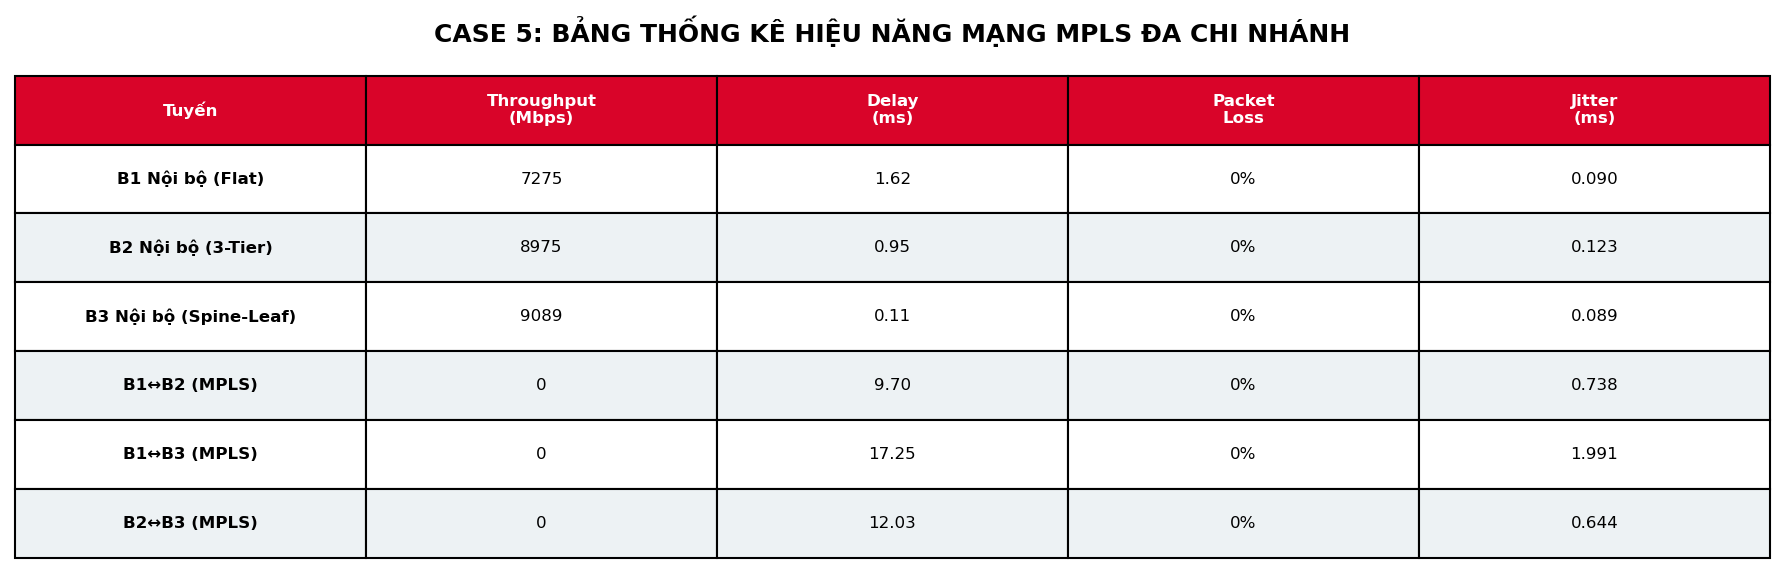
\includegraphics[width=0.9\textwidth]{image/case5_performance_table_gui.png}\\
        \vspace{0.2cm}
        
\includegraphics[width=0.9\textwidth]{image/packet_loss_chart.png}
    \end{columns}
\end{frame}

\section{Tổng kết}
\begin{frame}{Tổng kết}
    \begin{itemize}
        \item \textbf{Đạt được:} Triển khai thành công và chứng minh được cơ chế MPLS thực tế trên môi trường mạng diện rộng ảo hóa với Mininet. Tích hợp tốt các thiết kế chuẩn LAN (Flat, 3-Tier, Leaf-Spine).
        \item \textbf{Dữ liệu trung thực:} 100\% các thông số là kết quả benchmark thật, hỗ trợ báo cáo chuẩn học thuật IEEE.
        \item \textbf{Sáng tạo:} Cung cấp GUI hỗ trợ giám sát, đo lường theo kịch bản và sinh biểu đồ tự động.
    \end{itemize}
    \vspace{0.5cm}
    \centering
    \Large \textbf{XIN CHÂN THÀNH CẢM ƠN THẦY VÀ CÁC BẠN ĐÃ LẮNG NGHE!}
\end{frame}

\end{document}
